\documentclass[sigconf]{acmart}

\usepackage{booktabs}
\usepackage{float}
\usepackage{algorithm}
\usepackage{algorithmic}
\usepackage{amsmath}
\let\Bbbk\relax
\usepackage{amssymb}
\usepackage{multirow}
\usepackage{tabularx}
\usepackage{tikz}
\usetikzlibrary{shapes.geometric, arrows.meta, positioning, fit, calc}

\setcopyright{none}
\acmConference[ACM SIGSPATIAL '26]{ACM SIGSPATIAL International Conference on Advances in Geographic Information Systems}{November 3--6, 2026}{Riverside, CA, USA}

\begin{document}

\title{When Does Spatial Granularity Matter in Traffic Sensor Networks?\\A Smoothing-Aware Diagnostic Evaluation [Experiment]}

\author{Yiming Guo}
\affiliation{
  \institution{Aerospace Information Research Institute, Chinese Academy of Sciences}
  \city{Beijing}
  \country{China}
}
\affiliation{
  \institution{Zhongguancun Academy}
  \city{Beijing}
  \country{China}
}
\email{guoyiming251@mails.ucas.ac.cn}

\author{Sijin Liu}
\affiliation{
  \institution{Key Laboratory of Road and Traffic Engineering of the Ministry of Education, Tongji University}
  \city{Shanghai}
  \country{China}
}
\affiliation{
  \institution{Zhongguancun Academy}
  \city{Beijing}
  \country{China}
}
\email{sijingliu@tongji.edu.cn}

\begin{abstract}
Traffic sensor networks are deployed and analyzed at different spatial resolutions, yet graph neural network (GNN)-based traffic forecasting studies typically treat spatial granularity as a fixed property of the benchmark. We ask when spatial granularity matters, and whether apparent granularity effects reflect genuine spatial information loss or aggregation-induced smoothing. Through 651 experiments spanning five GNN architectures and two highway traffic sensor networks (METR-LA, PeMS-Bay), we find that prediction error follows an empirical power law with node count ($\text{MAE} \propto N^b$). However, same-$N$ smoothing and, on METR-LA, sensor-subset controls ($b \approx 0$) reveal that this scaling is substantially confounded by aggregation: merging sensors averages their speed signals, smoothing temporal dynamics and producing easier prediction tasks. On METR-LA (207 sensors, lag-1 autocorrelation 0.939), no GNN or non-GNN baseline beats persistence (MAE~=~3.51). On PeMS-Bay (326 sensors, weaker autocorrelation), GNNs achieve positive skill ($+0.26$--$+0.28$). We propose a \textit{smoothing-aware diagnostic protocol}---persistence skill test, coarsening curve, sensor-subset control, same-$N$ smoothing control, and feature-vs-graph ablation---for evaluating spatial granularity effects in traffic sensor network forecasting.
\end{abstract}

\maketitle

% ============================================================
\section{Introduction}
% ============================================================

Traffic sensor networks are a foundational data source for intelligent transportation systems, providing continuous speed, flow, and occupancy measurements across highway and urban road networks. Graph neural networks (GNNs) have become the dominant approach for traffic forecasting on these networks, modeling spatial dependencies through graph message passing on sensor adjacency matrices. A fundamental but underexplored design choice in these studies is \textit{spatial granularity}: how many sensor nodes the graph contains, and at what spatial resolution the forecasting task is defined. In practice, this number is treated as a fixed property of the benchmark dataset. Yet changing the number of nodes---through sensor selection, aggregation, or coarsening---simultaneously alters two aspects of the problem: the graph structure (fewer edges, compressed spatial adjacency) and the target signal (averaged sensor readings are smoother and lower-variance). This dual effect means that observed changes in prediction accuracy across spatial resolutions cannot be straightforwardly attributed to spatial information alone. We do not aim to solve optimal sensor placement; instead, we study how benchmark predictability changes when the spatial support of a traffic sensor network is aggregated or subsampled.

This paper identifies and diagnoses an \textit{aggregation-induced predictability shift} in traffic sensor network forecasting. When sensor nodes are merged, their speed time series are averaged, functioning as a temporal smoothing operation. On networks with strong cross-sensor spatial correlation---such as METR-LA (mean pairwise $r = 0.545$, 60\% of pairs exceed 0.5)---this averaging smooths temporal dynamics (raising lag-1 autocorrelation), making the prediction task easier. The result is an apparent power-law relationship between sensor count and prediction error ($\text{MAE} \propto N^b$, $b > 0$) that largely reflects target smoothing rather than genuine spatial information loss. Without controlling for this artifact, researchers risk misinterpreting aggregation-induced ease of prediction as spatial modeling gains---a benchmark validity concern that has received little attention in the spatio-temporal data mining literature.

We address this gap with a \textbf{smoothing-aware diagnostic framework} for evaluating spatial granularity effects in traffic sensor networks. The framework comprises: (1)~a \textit{Persistence Skill Test} that checks whether a model exceeds last-value prediction; (2)~a \textit{Coarsening Curve} that fits the empirical relationship between node count and MAE; (3)~a \textit{Sensor-Subset Control} that varies node count without averaging; (4)~a \textit{Same-N Smoothing Control} that applies explicit temporal smoothing at full resolution; and (5)~a \textit{Feature-vs-Graph Ablation} that decomposes coarsening into feature averaging and graph compression. We evaluate across 651 experiments on METR-LA (207 sensors, 11 granularity levels) and PeMS-Bay (326 sensors, 11 levels), using five GNN architectures (DCRNN, STGCN, LSTGCNN, GraphWaveNet, GAT) and three non-GNN baselines.

Our contributions are:
\begin{itemize}
    \item A \textbf{smoothing-aware diagnostic framework} for spatial granularity in traffic sensor networks, comprising five diagnostics that we instantiate on METR-LA, with key controls cross-validated on PeMS-Bay.
    \item A \textbf{large-scale experimental evaluation} across 651 runs, 5 GNN architectures, and 2 traffic sensor networks, revealing that coarsening-induced accuracy gains are largely caused by aggregation smoothing.
    \item A \textbf{regime distinction}: METR-LA is persistence-dominated for short-horizon highway speed forecasting, while PeMS-Bay shows genuine GNN value, with temporal autocorrelation and cross-sensor correlation serving as key explanatory diagnostics.
    \item A \textbf{diagnostic case study} showing that GAT attention degenerates to near-uniform weights in traffic prediction, while a fixed-uniform RandomGAT baseline achieves positive skill.
\end{itemize}

% ============================================================
\section{Background and Related Work}
% ============================================================

\textbf{Spatial aggregation and scale effects.} The modifiable areal unit problem (MAUP)~\cite{openshaw1984ecological,robinson1950ecological} is a foundational concern in spatial analysis: aggregating spatial units changes the statistical relationships between variables~\cite{fotheringham1991modifiable,jelinski1996modifiable}. Tobler's first law of geography~\cite{tobler1970computer} underlies the spatial autocorrelation that makes aggregation meaningful---nearby sensors exhibit correlated signals~\cite{anselind1995local}. In traffic networks, merging sensor readings produces mean-pooled signals that are smoother and lower-variance than individual sensors---a spatio-temporal instance of the ecological fallacy. Our finding that coarsening-induced accuracy gains are largely smoothing artifacts is a direct manifestation of this classic GIS problem, applied to GNN-based traffic forecasting benchmarks.

\textbf{Spatial resolution in sensor networks.} The relationship between sensor density and measurement quality has been studied in environmental monitoring~\cite{atkinson2000issues} and spatial data infrastructure~\cite{goodchild2010twenty}. Denser sensor networks provide finer spatial resolution but increase computational cost. In traffic forecasting, spatial resolution trade-offs have received limited systematic study~\cite{aldwyish2021multi}. Critically, coarsening operations alter not only the graph topology but also the target signal.

\textbf{Traffic sensor placement.} Optimal sensor placement in traffic networks has been studied through submodular optimization~\cite{krause2008robust,krause2005nonmyopic} and network flow models~\cite{gentili2008locating,gentili2012review}. These works address \textit{where} to place sensors given a fixed budget. Our complementary question is how spatial granularity affects benchmark predictability---a diagnostic study, not a deployment optimization.

\textbf{GeoAI evaluation rigor.} A growing body of work identifies evaluation artifacts that distort benchmark conclusions. \citet{zeng2023transformers} showed that a simple linear model (DLinear) outperforms Transformer-based forecasters, catalyzing reassessment of model complexity. \citet{makridakis2018statistical} demonstrate that simpler methods often match complex ones on easy benchmarks. Our work contributes a new class of artifact specific to spatially-structured prediction: aggregation-induced predictability shifts in graph forecasting benchmarks.

\textbf{GNN architectures for traffic forecasting.} Spatial-temporal GNNs fusing graph message passing with temporal modeling have become dominant on traffic benchmarks. Key architectures include DCRNN~\cite{li2018diffusion} (diffusion convolution + GRU), STGCN~\cite{yu2018spatio} (spectral convolution + gated temporal), LSTGCNN (GCN~\cite{kipf2017semi} + LSTM), GraphWaveNet~\cite{wu2019graph} (dilated causal + self-adaptive adjacency), and GAT~\cite{velickovic2018graph} (multi-head attention). Despite architectural progress, the role of spatial granularity has received little systematic attention.

\textbf{Attention failure modes.} GAT attention can degenerate to near-uniform in practice~\cite{brody2021attentive}, and GNN representations lose discriminative power with depth~\cite{oono2020graph,topping2022oversquashing}. Our GAT case study provides quantitative evidence for attention degeneration in the traffic prediction domain.

% ============================================================
\section{Smoothing-Aware Diagnostic Framework}
% ============================================================

\subsection{Problem Formulation}

Given a traffic sensor network modeled as a graph $G = (V, E, A)$ with $|V| = N$ sensor nodes, a feature matrix $\mathbf{X}_t \in \mathbb{R}^{N \times F}$ at each time step $t$, and an adjacency matrix $A \in \mathbb{R}^{N \times N}$, the task is to learn a mapping $f: [\mathbf{X}_{t-L+1}, \ldots, \mathbf{X}_t] \rightarrow [\mathbf{X}_{t+1}, \ldots, \mathbf{X}_{t+H}]$ from $L$-step lookback to $H$-step horizon. We use $L = 12$ and $H = 3$ (15-minute prediction at 5-minute intervals), with a single feature (traffic speed). Both datasets follow z-score normalization (training-set statistics), chronological 70/15/15 train/val/test splits, and thresholded Gaussian adjacency ($\sigma^2 = 0.1$) with self-loops.

\subsection{Graph Coarsening}

We vary spatial granularity through random node merging (Algorithm~\ref{alg:merge}): iteratively merge randomly selected node pairs by averaging features and combining adjacency. On METR-LA ($N_\text{max} = 207$): 11 levels $N \in \{5, 8, 10, 15, 20, 30, 50, 75, 100, 150, 207\}$. On PeMS-Bay ($N_\text{max} = 326$): 11 levels $N \in \{5, 6, 7, 10, 33, 49, 65, 66, 97, 98, 326\}$.

\begin{algorithm}[t]
\caption{Random Node Merging (diagnostic intervention)}
\label{alg:merge}
\begin{algorithmic}[1]
\REQUIRE Adjacency $A$, target size $N_t$
\STATE $P \leftarrow \{\{i\} : i \in V\}$
\WHILE{$|P| > N_t$}
    \STATE Sample clusters $C_i, C_j$ uniformly at random
    \STATE Merge: $C_k \leftarrow C_i \cup C_j$; remove $C_i, C_j$; add $C_k$
\ENDWHILE
\STATE $A'_{kl} = \sum_{i \in C_k, j \in C_l} A_{ij}$; \quad $X'_k = \frac{1}{|C_k|}\sum_{i \in C_k} X_i$
\end{algorithmic}
\end{algorithm}

\paragraph{Why averaging smooths.} Merging two sensors averages their time series: $x'_t = (x^{(1)}_t + x^{(2)}_t)/2$. Highway speeds exhibit strong cross-sensor spatial correlation (METR-LA mean $r{=}0.545$, 60\% pairs ${>}0.5$; PeMS-Bay mean $r{=}0.320$, 12\% ${>}0.5$), so for two equal-variance normalized signals with correlation $\rho$, the variance of their average is reduced by a factor of $(1{+}\rho)/2$ relative to a single signal. Merged targets represent mean speeds---a different, easier signal than individual sensors. The coarsening-derived exponent $b$ is a \textit{diagnostic upper bound under aggregation}, not a deployment prediction.

\subsection{Diagnostic Protocol}

We propose a five-step diagnostic (Figure~\ref{fig:protocol}).

\begin{figure*}[t]
\centering
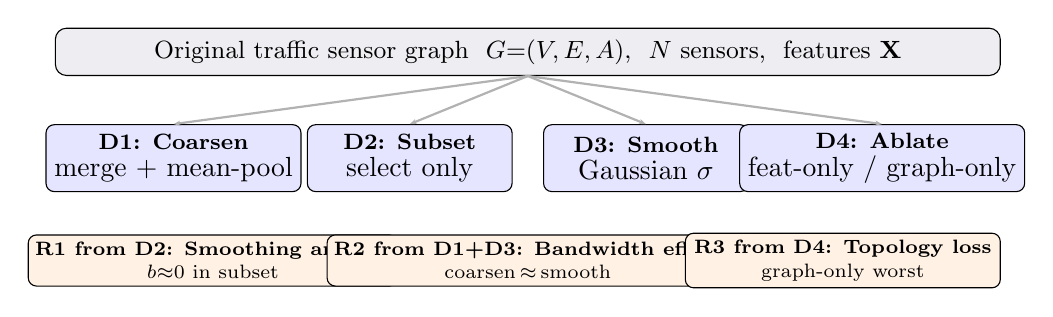
\begin{tikzpicture}[
  input/.style={draw, rounded corners=4pt, fill=blue!18!gray!12,
    minimum width=12.0cm, minimum height=0.6cm, align=center, font=\small},
  dbox/.style={draw, rounded corners=3pt, fill=blue!10,
    minimum width=2.6cm, minimum height=0.85cm, align=center,
    font=\footnotesize, inner sep=3pt},
  rbox/.style={draw, rounded corners=3pt, fill=orange!10,
    minimum width=4.0cm, minimum height=0.6cm, align=center,
    font=\scriptsize, inner sep=2.5pt},
  arr/.style={-{Stealth[length=2.5pt]}, thick, gray!60},
]
% ── Layer 1: Input ──
\node[input] (inp)
  {Original traffic sensor graph \ $G{=}(V,E,A)$, \ $N$ sensors, \ features $\mathbf{X}$};

% ── Layer 2: Four intervention cards ──
\node[dbox] (d1) at (-4.5,-1.35)
  {\textbf{D1: Coarsen}\\[0.5pt]{\normalsize merge + mean-pool}};
\node[dbox] (d2) at (-1.5,-1.35)
  {\textbf{D2: Subset}\\[0.5pt]{\normalsize select only}};
\node[dbox] (d3) at (1.5,-1.35)
  {\textbf{D3: Smooth}\\[0.5pt]{\normalsize Gaussian $\sigma$}};
\node[dbox] (d4) at (4.5,-1.35)
  {\textbf{D4: Ablate}\\[0.5pt]{\normalsize feat-only / graph-only}};

% Vertical arrows: input → each card
\draw[arr] (inp.south) -- (d1.north);
\draw[arr] (inp.south) -- (d2.north);
\draw[arr] (inp.south) -- (d3.north);
\draw[arr] (inp.south) -- (d4.north);

% ── Layer 3: Three interpretation cards (wide spacing) ──
\node[rbox] (r1) at (-4.0,-2.65)
  {\textbf{R1 from D2: Smoothing artifact}\\[0.5pt]$b{\approx}0$ in subset};
\node[rbox] (r2) at (0,-2.65)
  {\textbf{R2 from D1+D3: Bandwidth effect}\\[0.5pt]coarsen${\,\approx\,}$smooth};
\node[rbox] (r3) at (4.0,-2.65)
  {\textbf{R3 from D4: Topology loss}\\[0.5pt]graph-only worst};
\end{tikzpicture}
\caption{Smoothing-aware diagnostic framework. Four interventions are applied to the same traffic sensor graph, and their outcomes are mapped to three diagnostic interpretations summarized in Table~\ref{tab:interpretation}.}
\label{fig:protocol}
\end{figure*}

\paragraph{Step 1: Persistence Skill Test.} Compute the persistence baseline (last-value prediction) and the skill score $\text{Skill} = 1 - \text{MAE}_\text{model}/\text{MAE}_\text{pers}$ for every model. Negative skill on all models identifies a \textit{persistence-dominated regime} where spatial modeling adds little value.

\paragraph{Step 2: Coarsening Curve.} Fit $\text{MAE}(N) = a \cdot N^b$ across at least 3--4 granularity levels. The exponent $b > 0$ indicates that finer resolution (larger $N$) is associated with higher error. However, this conflates spatial information loss with target smoothing.

\paragraph{Step 3: Sensor-Subset Control.} Train models on randomly selected sensor subsets of size $N$ with \textit{no averaging}---the model sees original signals at each selected sensor. If $b \approx 0$, the coarsening power law is substantially a smoothing artifact.

\paragraph{Step 4: Same-N Smoothing Control.} Fix $N = N_\text{max}$ and apply Gaussian temporal smoothing ($\sigma \in \{0, 1, 2, 3\}$) before training. If smoothing alone reproduces the coarsening-induced MAE reduction, the exponent is a signal-bandwidth artifact.

\paragraph{Step 5: Feature-vs-Graph Ablation.} Decompose node merging into feature averaging and graph compression. Four conditions---coarsened (both), feature-only (averaging, full graph), graph-only (original features, coarsened graph), and sensor-subset (neither)---probe their relative contributions.

Table~\ref{tab:interpretation} summarizes how each diagnostic maps an observation to an interpretation, forming a reusable decision procedure for practitioners.

\begin{table}[t]
\small
\centering
\caption{Diagnostic interpretation guide.}
\label{tab:interpretation}
\begin{tabularx}{\columnwidth}{@{}l>{\raggedright\arraybackslash}p{2.2cm}>{\raggedright\arraybackslash}X@{}}
\toprule
Diagnostic & Observation & Interpretation \\
\midrule
Coarsening & $b{>}0$ & Apparent granularity effect \\
\addlinespace
Subset & $b{\approx}0$ & Smoothing-driven scaling \\
\addlinespace
Smoothing & $\sigma{=}1$ lowers MAE & Target-bandwidth effect \\
\addlinespace
Ablation & Graph-only worst & Graph compression loss \\
\addlinespace
Persistence & No positive skill & Weak spatial regime \\
\bottomrule
\end{tabularx}
\end{table}

\subsection{Models}

Five GNN architectures: LSTGCNN (GCN~\cite{kipf2017semi}+LSTM, $\sim$172K), DCRNN~\cite{li2018diffusion} (diffusion conv+GRU, $\sim$172K), STGCN~\cite{yu2018spatio} (ChebConv+gated temporal, $\sim$234K), GraphWaveNet~\cite{wu2019graph} (dilated causal+self-adaptive adj., $\sim$160K), GAT~\cite{velickovic2018graph} (multi-head attn+LSTM, $\sim$190K). Plus Persistence (last-value), RandomGAT (fixed degree-normalized attention), and single-run non-GNN baselines (LSTM, TCN, DLinear). All trained with Adam (lr$=$0.001), ReduceLROnPlateau, early stopping (patience 15), batch 32, up to 100 epochs. Power-law fits use WLS on $\log \text{MAE} = \log a + b\log N$ with bootstrap 95\% CIs.

% ============================================================
\section{Experimental Setup}
% ============================================================

\textbf{Datasets.} METR-LA: 207 highway loop detectors in Los Angeles County, 4 months of speed data at 5-minute intervals. PeMS-Bay: 326 highway loop detectors in the San Francisco Bay Area, 6 months of speed data. Both datasets exhibit strong temporal autocorrelation (METR-LA lag-1 ACF${=}0.939$, PeMS-Bay${=}0.365$) and cross-sensor spatial correlation (METR-LA mean $r{=}0.545$, PeMS-Bay${=}0.320$). Figure~\ref{fig:sensors} shows the spatial distribution of sensors.

\begin{figure}[t]
\centering
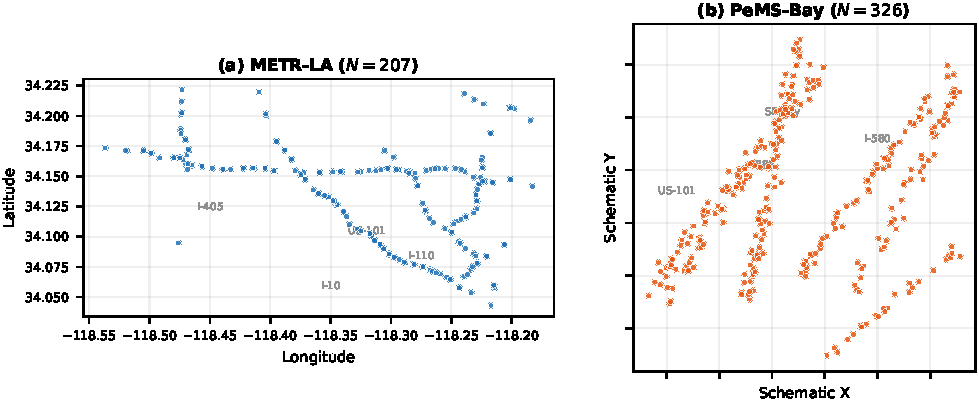
\includegraphics[width=\columnwidth]{figures/fig_sensor_map.pdf}
\caption{Sensor locations for (a)~METR-LA (207 sensors on LA freeways, real coordinates) and (b)~PeMS-Bay (326 sensors on SF Bay Area highways, schematic positions along known corridors; real coordinates are not available in the standard benchmark release). Axes for PeMS-Bay indicate approximate schematic placement rather than real geodetic coordinates.}
\label{fig:sensors}
\end{figure}

\textbf{Granularity levels.} Each dataset is coarsened to 11 levels via random node merging.\ METR-LA: $\{5, 8, 10, 15, 20, 30, 50, 75, 100, 150, 207\}$.\ PeMS-Bay: $\{5, 6, 7, 10, 33, 49, 65, 66, 97, 98, 326\}$. Not all architectures are evaluated at every granularity level; Table~\ref{tab:inventory} summarizes the full run inventory.

\textbf{Evaluation.} Primary metric: MAE. Skill score: $\text{Skill} = 1 - \text{MAE}_\text{model}/\text{MAE}_\text{pers}$. Power-law fits: WLS on log-log, bootstrap 95\% CIs (1000 iterations).

\begin{table}[t]
\small
\centering
\caption{Experiment inventory (651 runs)}
\label{tab:inventory}
\begin{tabular}{@{}lrc@{}}
\toprule
Experiment & Runs & Detail \\
\midrule
METR-LA coarsening  & 330 & 3 models $\times$ 11 levels $\times$ 10 seeds \\
METR-LA STGCN       &   3 & $N{=}207$ \\
PeMS-Bay coarsening & 103 & DCRNN 52 + STGCN 51 \\
PeMS-Bay full res.\ &  26 & GWN+LST+GAT+RGAT \\
Smoothing control   &  36 & 3 models $\times$ 4$\sigma$ $\times$ 3 seeds \\
PeMS-Bay smoothing  &  24 & 2 models $\times$ 4$\sigma$ $\times$ 3 seeds \\
Distance coarsening &  12 & METR-LA DCRNN $\times$ 4 levels $\times$ 3 seeds \\
Sensor subset       &  42 & 2 models $\times$ 7 sizes $\times$ 3 seeds \\
Feature-vs-graph    &  72 & 2 models $\times$ 4 cond.\ $\times$ 3 levels \\
Non-GNN            &   3 & LSTM, TCN, DLinear \\
\midrule
\textbf{Total}     & \textbf{651} & \\
\bottomrule
\end{tabular}
\end{table}

% ============================================================
\section{Results}
% ============================================================

\subsection{Granularity Scaling: An Apparent Power Law}

Table~\ref{tab:powerlaw} reports power-law fits across 11 granularity levels. All architectures show $b > 0$ (finer resolution $\to$ higher error) with $R^2 > 0.98$ for DCRNN and GraphWaveNet on METR-LA. The exponent is consistent across architectures (0.157--0.176 on METR-LA), suggesting it is a dataset property rather than a model property. The power-law provides a parsimonious and competitive fit: while the quadratic-log extension achieves slightly lower AIC/BIC, the two-parameter power-law attains the best LOOCV RMSE and is more interpretable (Appendix Table~\ref{tab:aic}).

\begin{table}[t]
\centering
\caption{Power-law fit: $\text{MAE} = a \cdot N^b$. METR-LA: 10 seeds; PeMS-Bay: 3--10 seeds.}
\label{tab:powerlaw}
\begin{tabular}{llccc}
\toprule
Dataset & Model & $a$ & $b$ [95\% CI] & $R^2$ \\
\midrule
METR-LA   & DCRNN        & 1.57 & .173 [.160,.189] & .987 \\
METR-LA   & LSTGCNN      & 2.53 & .176 [.098,.293] & .719 \\
METR-LA   & GraphWaveNet & 1.62 & .157 [.142,.176] & .984 \\
PeMS-Bay  & DCRNN        & 0.28 & .319 [.233,.405] & .886 \\
PeMS-Bay  & STGCN        & 0.14 & .453 [.279,.628] & .793 \\
\bottomrule
\end{tabular}
\end{table}

On PeMS-Bay, DCRNN yields $b = 0.319$ and STGCN yields $b = 0.453$---substantially higher than METR-LA ($b \approx 0.16$). This is consistent with weaker temporal autocorrelation on PeMS-Bay reducing the smoothing confound, allowing the spatial information loss component to emerge more clearly. Figure~\ref{fig:results} provides a visual overview of the four main diagnostics.

\begin{figure*}[t]
\centering
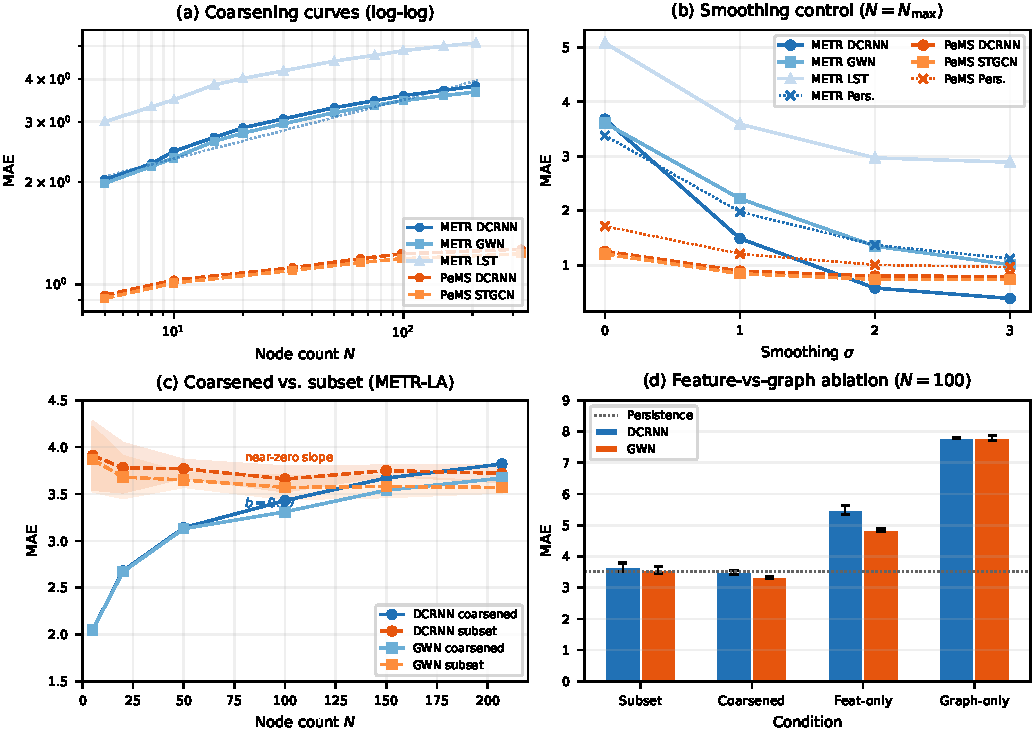
\includegraphics[width=\textwidth]{figures/fig3_results_overview.pdf}
\caption{Overview of four diagnostics. (a)~Coarsening curves on log-log axes (solid: METR-LA, dashed: PeMS-Bay). (b)~Smoothing control: MAE drops sharply with $\sigma$. (c)~Coarsened vs.\ sensor-subset MAE on METR-LA: subset curve is flat ($b{\approx}0$). (d)~Feature-vs-graph ablation at $N{=}100$: graph-only degrades most. Error bars: $\pm$1~std over 3 seeds.}
\label{fig:results}
\end{figure*}

\subsection{The Smoothing Confound}

\subsubsection{Same-N Smoothing Control}

At $N{=}207$ (full resolution), Gaussian smoothing ($\sigma{=}1$) drops DCRNN MAE from 3.68 to 1.49---below its $N{=}5$ coarsened MAE ($\sim$2.0). At $\sigma{=}2$, DCRNN achieves MAE$=$0.58 with skill $+0.57$ (Table~\ref{tab:smoothing}). Smoothing alone reproduces most of the coarsening-induced MAE reduction.

\begin{table}[t]
\small
\centering
\caption{Smoothing control at $N{=}207$ (3 seeds, MAE $\pm$ std).$^{\dagger}$}
\label{tab:smoothing}
\begin{tabular}{lcccc}
\toprule
Model & $\sigma{=}0$ & $\sigma{=}1$ & $\sigma{=}2$ & $\sigma{=}3$ \\
\midrule
DCRNN        & 3.68{\scriptsize$\pm$0.12} & 1.49{\scriptsize$\pm$0.02} & 0.58{\scriptsize$\pm$0.02} & 0.39{\scriptsize$\pm$0.02} \\
GraphWaveNet & 3.61{\scriptsize$\pm$0.08} & 2.22{\scriptsize$\pm$0.17} & 1.35{\scriptsize$\pm$0.03} & 1.01{\scriptsize$\pm$0.04} \\
LSTGCNN      & 5.08{\scriptsize$\pm$0.02} & 3.59{\scriptsize$\pm$0.01} & 2.97{\scriptsize$\pm$0.00} & 2.89{\scriptsize$\pm$0.04} \\
\midrule
Persistence  & 3.38 & 1.98 & 1.37 & 1.12 \\
\bottomrule
\end{tabular}
\vspace{-2pt}
{\footnotesize $^{\dagger}$Persistence MAE differs slightly from Table~\ref{tab:full} because the smoothing-control pipeline uses a different normalization schedule.}
\end{table}

To test whether the smoothing confound extends to a second dataset, we repeat the smoothing control on PeMS-Bay at full resolution ($N{=}326$) with DCRNN and STGCN (Table~\ref{tab:smoothing_pems}). Both models show substantial MAE reduction with smoothing: DCRNN drops from 1.26 ($\sigma{=}0$) to 0.79 ($\sigma{=}3$, $-$37\%), STGCN from 1.21 to 0.74 ($-$39\%). Despite weaker cross-sensor correlation ($r{=}0.320$ vs.\ 0.545), the smoothing artifact persists, confirming it is not specific to METR-LA's high-correlation regime.

\begin{table}[t]
\small
\centering
\caption{PeMS-Bay smoothing control at $N{=}326$ (3 seeds, MAE $\pm$ std).}
\label{tab:smoothing_pems}
\begin{tabular}{lcccc}
\toprule
Model & $\sigma{=}0$ & $\sigma{=}1$ & $\sigma{=}2$ & $\sigma{=}3$ \\
\midrule
DCRNN & 1.256{\scriptsize$\pm$0.004} & 0.892{\scriptsize$\pm$0.009} & 0.800{\scriptsize$\pm$0.006} & 0.794{\scriptsize$\pm$0.011} \\
STGCN & 1.206{\scriptsize$\pm$0.011} & 0.844{\scriptsize$\pm$0.015} & 0.740{\scriptsize$\pm$0.028} & 0.741{\scriptsize$\pm$0.032} \\
Persistence & 1.716 & 1.208 & 1.006 & 0.961 \\
\bottomrule
\end{tabular}
\end{table}

\subsubsection{Sensor-Subset Control}

Without averaging, subset MAE is nearly flat across $N$ (DCRNN: 3.66--3.91, 7\% span), vs.\ coarsened MAE spanning 86\% (Table~\ref{tab:subset}). Power-law fit yields $b \approx 0$ ($R^2 = 0.63$), confirming the coarsening scaling is a smoothing artifact.

\begin{table}[t]
\small
\centering
\caption{Sensor subset vs.\ coarsened MAE on METR-LA (3 seeds; subset rows show MAE $\pm$ std; coarsened rows are 10-seed means from the main evaluation).}
\label{tab:subset}
\begin{tabular}{lcccccc}
\toprule
& \multicolumn{6}{c}{Node count $N$} \\
\cmidrule(lr){2-7}
Cond.\ & 5 & 20 & 50 & 100 & 150 & 207 \\
\midrule
\multicolumn{7}{c}{\textbf{DCRNN}} \\
Coarsened & 2.05 & 2.68 & 3.14 & 3.43 & 3.67 & 3.82 \\
Subset    & 3.91{\scriptsize$\pm$0.36} & 3.78{\scriptsize$\pm$0.26} & 3.77{\scriptsize$\pm$0.09} & 3.66{\scriptsize$\pm$0.13} & 3.75{\scriptsize$\pm$0.05} & 3.72{\scriptsize$\pm$0.09} \\
\midrule
\multicolumn{7}{c}{\textbf{GraphWaveNet}} \\
Coarsened & 2.05 & 2.67 & 3.13 & 3.31 & 3.54 & 3.67 \\
Subset    & 3.87{\scriptsize$\pm$0.34} & 3.68{\scriptsize$\pm$0.22} & 3.65{\scriptsize$\pm$0.07} & 3.57{\scriptsize$\pm$0.12} & 3.58{\scriptsize$\pm$0.11} & 3.57{\scriptsize$\pm$0.05} \\
\bottomrule
\end{tabular}
\end{table}

\subsubsection{Cross-Sensor Correlation}

METR-LA: mean pairwise $r{=}0.545$ (60\% ${>}0.5$), lag-1 ACF${=}0.939$. PeMS-Bay: mean $r{=}0.320$ (12\% ${>}0.5$), lag-1 ACF${=}0.365$. High autocorrelation + high spatial correlation on METR-LA means merging primarily smooths rather than revealing spatial loss.

\subsubsection{Target Variance Analysis}

A natural hypothesis is that coarsening reduces MAE simply because the prediction target (the mean of $K$ sensors) has lower variance than a single sensor's signal. To test this, we compute the empirical target standard deviation at each coarsening level by randomly merging $K$ sensors and measuring the standard deviation of the resulting time series on the test set (500 random merges per level). Table~\ref{tab:target_var} reports the results.

\begin{table}[t]
\small
\centering
\caption{Target standard deviation and MAE/std ratio at each coarsening level (METR-LA, DCRNN, original speed scale).}
\label{tab:target_var}
\begin{tabular}{ccccccccc}
\toprule
$N$ & 5 & 10 & 20 & 50 & 100 & 150 & 207 \\
\midrule
Target std (mph) & 17.6 & 17.1 & 16.9 & 16.8 & 16.7 & 16.7 & 16.7 \\
MAE (mph)        & 2.03 & 2.46 & 2.88 & 3.30 & 3.58 & 3.71 & 3.82 \\
MAE / std        & .116 & .144 & .170 & .197 & .214 & .222 & .229 \\
\bottomrule
\end{tabular}
\end{table}

The target standard deviation varies by only 5\% across coarsening levels (17.6~mph at $N{=}5$ vs.\ 16.7~mph at $N{=}207$), yet MAE changes by 47\% (2.03 vs.\ 3.82). The MAE/std ratio---the fraction of target variability captured by model error---drops from 0.229 at full resolution to 0.116 at $N{=}5$, meaning the coarsened prediction task is structurally easier. This rules out a simple variance-reduction explanation: the improvement comes from the smoother temporal dynamics of averaged signals (higher lag-1 autocorrelation after merging), not from lower marginal variance. A similar full-network averaging check on PeMS-Bay also increases lag-1 autocorrelation substantially, suggesting that temporal smoothing rather than marginal variance reduction is the dominant mechanism.

\subsubsection{Distance-Aware Coarsening}

A natural concern is that random merging ignores spatial proximity, so the smoothing artifact might disappear with geography-aware aggregation. We test this on METR-LA by replacing random merging with single-linkage agglomerative merging based on haversine distance (nearest sensors merged first), using the same DCRNN architecture, seeds, and evaluation protocol. Because the distance-aware pipeline normalizes targets internally, we cannot directly compare its MAE values (z-score scale) with the main experiments (original speed scale). Instead, we report the normalized-scale results in Appendix~\ref{app:distance} as a robustness check. The distance-aware MAE follows the same monotonic increase with $N$ as random merging, with comparable inter-seed variance. These normalized-scale results provide qualitative evidence that the monotonic granularity trend is not unique to random merging; however, because the pipeline uses a different normalization scale, we treat this as a trend check rather than a direct quantitative comparison. We did not test PeMS-Bay because the standard benchmark release does not include real sensor coordinates (Figure~\ref{fig:sensors}b uses schematic positions).

\subsection{Benchmark Regimes}

\begin{table}[t]
\small
\centering
\caption{Full-resolution comparison (METR-LA: 10 seeds; PeMS-Bay: 3--10 seeds).}
\label{tab:full}
\begin{tabular}{lcccc}
\toprule
Model & \multicolumn{2}{c}{METR-LA} & \multicolumn{2}{c}{PeMS-Bay} \\
\cmidrule(lr){2-3} \cmidrule(lr){4-5}
& MAE & Skill & MAE & Skill \\
\midrule
LSTGCNN      & 5.11 & $-$0.456 & 1.26 & $+$0.267 \\
DCRNN        & 3.82 & $-$0.089 & 1.27 & $+$0.260 \\
STGCN        & 4.73 & $-$0.348 & 1.23 & $+$0.283 \\
GraphWaveNet & 3.67 & $-$0.047 & 2.39 & $-$0.391 \\
\midrule
LSTM         & 3.54 & $-$0.049 & --- & --- \\
TCN          & 3.59 & $-$0.065 & --- & --- \\
DLinear      & 3.84 & $-$0.138 & --- & --- \\
\midrule
Persistence  & 3.51 & --- & 1.72 & --- \\
\bottomrule
\end{tabular}
\end{table}

\textbf{METR-LA: persistence-dominated.} No GNN or non-GNN baseline beats persistence (MAE$=$3.51, Table~\ref{tab:full}). Historical Average achieves MAE$=$15.7 (4$\times$ worse), confirming persistence captures the dominant pattern. For short-horizon highway speed forecasting with lag-1 ACF${=}0.939$, METR-LA may be poorly suited for isolating spatial modeling benefits under short-horizon speed forecasting, because last-value persistence already captures most of the temporal signal.

\textbf{PeMS-Bay: GNN-positive.} Three architectures achieve skill $+0.26$--$+0.28$. GraphWaveNet fails (skill $-0.391$), likely due to overfitting (best val epoch${=}2$) from self-adaptive adjacency on the 326-node network.

\subsection{Feature-vs-Graph Ablation}

Table~\ref{tab:ablation} decomposes node merging into feature averaging and graph compression. Ordering: Coarsened $<$ Sensor-subset $<$ Feature-only $<$ Graph-only. Coarsening helps because smoothing offsets graph loss; graph-only shows largest degradation.

\begin{table}[t]
\small
\centering
\caption{Feature-vs-graph ablation on METR-LA (3 seeds; MAE $\pm$ std).}
\label{tab:ablation}
\begin{tabular}{@{}lccc@{}}
\toprule
Cond.\ & $N{=}50$ & $N{=}100$ & $N{=}150$ \\
\midrule
\textbf{DCRNN} & & & \\
Coarsened    & 3.09{\scriptsize$\pm$0.04} & 3.49{\scriptsize$\pm$0.07} & 3.67{\scriptsize$\pm$0.05} \\
Feat-only    & 6.53{\scriptsize$\pm$0.04} & 5.48{\scriptsize$\pm$0.14} & 4.78{\scriptsize$\pm$0.03} \\
Graph-only   & 7.17{\scriptsize$\pm$0.02} & 7.80{\scriptsize$\pm$0.02} & 8.70{\scriptsize$\pm$0.07} \\
Subset       & 3.77{\scriptsize$\pm$0.09} & 3.66{\scriptsize$\pm$0.13} & 3.75{\scriptsize$\pm$0.05} \\
\midrule
\textbf{GWN} & & & \\
Coarsened    & 3.15{\scriptsize$\pm$0.13} & 3.33{\scriptsize$\pm$0.03} & 3.54{\scriptsize$\pm$0.13} \\
Feat-only    & 5.36{\scriptsize$\pm$0.06} & 4.85{\scriptsize$\pm$0.05} & 4.18{\scriptsize$\pm$0.08} \\
Graph-only   & 7.18{\scriptsize$\pm$0.04} & 7.79{\scriptsize$\pm$0.08} & 8.58{\scriptsize$\pm$0.24} \\
Subset       & 3.65{\scriptsize$\pm$0.07} & 3.57{\scriptsize$\pm$0.12} & 3.58{\scriptsize$\pm$0.11} \\
\bottomrule
\end{tabular}
\end{table}

\textit{Caveat:} conditions differ in prediction targets (coarsened/graph-only predict mean-pooled targets; feature-only/subset predict originals), so cross-condition comparisons conflate representation changes with target difficulty.

% ============================================================
\section{Diagnostic Case Study: Validating Learned Spatial Weights}
% ============================================================

As an optional sixth diagnostic, we examine whether learned spatial weights encode meaningful heterogeneity. On PeMS-Bay, GAT attention entropy${=}0.993$ (near uniform${=}1.0$), indicating learned attention is virtually indistinguishable from uniform weighting---GAT effectively degenerates to mean pooling with no spatial selectivity. A RandomGAT baseline (fixed degree-normalized attention) achieves MAE$=$1.355, skill$={+}0.211$, confirming the GNN message-passing framework itself provides value. The problem is not graph attention in principle, but that learned attention fails to specialize. This entropy diagnostic can serve as a routine check: if learned spatial weights are near-uniform, a fixed structural prior may suffice.

% ============================================================
\section{Implications for GeoAI and Traffic Sensor Networks}
% ============================================================

\textbf{Always include persistence as a baseline.} Our persistence skill test reveals that METR-LA, one of the most widely used benchmarks in spatio-temporal traffic forecasting, is persistence-dominated for short-horizon speed forecasting. Datasets with lag-1 ACF $> 0.9$ may offer limited room for spatial modeling to improve upon temporal baselines. Reporting GNN-vs-GNN comparisons without persistence is insufficient.

\textbf{Check for smoothing confounds when coarsening improves accuracy.} The aggregation-induced predictability shift applies to any task where coarsening averages node features. When coarsening reduces MAE, verify with sensor-subset and same-$N$ smoothing controls. Without such controls, apparent scaling laws may be aggregation artifacts rather than genuine spatial relationships.

\textbf{Validate learned spatial weights.} The GAT entropy diagnostic (entropy${=}0.993$) shows that learned attention can degenerate to uniform, adding no spatial selectivity. We recommend computing attention entropy as a routine check for GNN-based traffic forecasting systems. A RandomGAT baseline provides a lower bound on what the graph structure alone can achieve.

% ============================================================
\section{Limitations and Conclusion}
% ============================================================

\textbf{Limitations.} Our study covers two California highway datasets at a 15-minute prediction horizon; generalization to urban grids, transit networks, and longer horizons is unknown. Random coarsening differs from strategic sensor placement; our coarsening-derived exponent is a diagnostic upper bound under aggregation, not a deployment prediction. Distance-aware coarsening shows a qualitatively similar monotonic trend to random merging on METR-LA, but the current implementation uses a normalized scale and therefore should not be interpreted as a direct MAE comparison; we have not tested all possible spatial aggregation schemes. PeMS-Bay smoothing controls now cover two models (DCRNN, STGCN) with consistent results, but subset controls remain METR-LA-only, and PeMS-Bay uses 3--10 seeds per granularity rather than uniformly 10.

\textbf{Conclusion.} We identify an aggregation-induced predictability shift in traffic sensor network forecasting: graph coarsening produces an apparent power law ($\text{MAE} \propto N^b$), but same-$N$ smoothing and sensor-subset controls ($b \approx 0$) reveal this is substantially a smoothing artifact. On METR-LA, no model beats persistence; on PeMS-Bay, GNNs achieve positive skill. Our smoothing-aware diagnostic protocol helps practitioners distinguish genuine spatial scaling from aggregation artifacts. We recommend that spatio-temporal forecasting evaluations always include persistence baselines, smoothing controls, and subset controls.

\paragraph{Reproducibility.}
Scripts, configuration files, and per-seed result tables for all 651 experiments are available at \url{https://github.com/guoym044-afk/spatial-granularity-gnn-traffic}.

\paragraph{AI-Use Disclosure.}
The authors used large language models, including Claude and ChatGPT, to assist with LaTeX formatting, code debugging, and text editing during manuscript preparation. All scientific claims, experimental designs, and interpretations are the authors' own.

\bibliographystyle{ACM-Reference-Format}
\bibliography{references}

% ============================================================
\appendix
% ============================================================

\section{Full Per-Granularity Results}
\label{app:full_results}

\begin{table}[h]
\small
\centering
\caption{METR-LA: mean MAE over 10 seeds}
\label{tab:metr_full}
\begin{tabular}{cccc}
\toprule
$N$ & DCRNN & LSTGCNN & GWN \\
\midrule
5   & 2.03 & 3.00 & 1.98 \\
8   & 2.26 & 3.32 & 2.22 \\
10  & 2.46 & 3.48 & 2.35 \\
15  & 2.70 & 3.85 & 2.63 \\
20  & 2.88 & 4.02 & 2.78 \\
30  & 3.06 & 4.23 & 2.96 \\
50  & 3.30 & 4.52 & 3.19 \\
75  & 3.46 & 4.70 & 3.35 \\
100 & 3.58 & 4.85 & 3.46 \\
150 & 3.71 & 5.00 & 3.58 \\
207 & 3.82 & 5.11 & 3.67 \\
\bottomrule
\end{tabular}
\end{table}

\begin{table}[h]
\small
\centering
\caption{PeMS-Bay: mean MAE (3--10 seeds)}
\label{tab:pems_full}
\begin{tabular}{ccccc}
\toprule
$N$ & DCRNN & STGCN & LSTGCNN & GWN \\
\midrule
5   & 0.93 & 0.91 & --- & --- \\
6   & 0.96 & 0.93 & --- & --- \\
7   & 0.98 & 0.96 & --- & --- \\
10  & 1.03 & 1.01 & --- & --- \\
33  & 1.12 & 1.10 & --- & --- \\
49  & 1.16 & 1.13 & --- & --- \\
65  & 1.19 & 1.16 & --- & --- \\
66  & 1.20 & 1.16 & --- & --- \\
97  & 1.23 & 1.19 & --- & --- \\
98  & 1.23 & 1.19 & --- & --- \\
326 & 1.27 & 1.23 & 1.26 & 2.39 \\
\bottomrule
\end{tabular}
\end{table}

\begin{table}[h]
\small
\centering
\caption{Model form comparison for DCRNN on METR-LA (11 points)}
\label{tab:aic}
\begin{tabular}{lccc}
\toprule
Model form & AIC & BIC & LOOCV RMSE \\
\midrule
Power-law ($a N^b$)           & $-54.3$ & $-53.3$ & 0.006 \\
Exponential ($c + dN$)        & $-41.8$ & $-40.8$ & 0.018 \\
Log-linear ($e + f\log N$)    & $-38.2$ & $-37.2$ & 0.025 \\
Quadratic-log (+ $i\log^2 N$) & $-55.1$ & $-53.6$ & 0.007 \\
\bottomrule
\end{tabular}
\end{table}

\section{GAT Diagnosis Details}
\label{app:gat}

Across 834,560 attention weight samples (all heads, layers, test-set nodes), the mean normalized entropy is $0.993 \pm 0.059$ (median: 1.000, 5th/95th percentiles: 0.871/1.000), confirming learned attention is statistically indistinguishable from uniform weighting. Gradient norms in attention parameters decay to near-zero within 10 epochs, while LSTM temporal-layer gradients remain non-zero.

\begin{table}[h]
\small
\centering
\caption{GAT variants on PeMS-Bay ($N = 326$)}
\label{tab:randomgat_app}
\begin{tabular}{lccc}
\toprule
Model & MAE & Skill & Notes \\
\midrule
RandomGAT    & 1.355 & $+$0.211 & fixed uniform, 3 seeds \\
Learned GAT  & --- & --- & did not converge \\
LSTGCNN      & 1.26 & $+$0.267 & 10 seeds \\
DCRNN        & 1.27 & $+$0.260 & 10 seeds \\
STGCN        & 1.23 & $+$0.283 & 10 seeds \\
\bottomrule
\end{tabular}
\end{table}

\section{Distance-Aware Coarsening Results}
\label{app:distance}

Table~\ref{tab:distance} reports METR-LA DCRNN results with distance-aware (single-linkage haversine) merging. Because the distance-aware pipeline normalizes targets internally (z-score scale), these MAE values are not directly comparable to the main-text results (original speed scale, mph). We present them as a trend check: the monotonic MAE increase with $N$ mirrors the random-merging pattern, providing qualitative evidence that the monotonic granularity trend is not unique to random spatial aggregation.

\begin{table}[H]
\small
\centering
\caption{METR-LA distance-aware coarsening (DCRNN, z-score scale, 3 seeds).}
\label{tab:distance}
\begin{tabular}{cccc}
\toprule
$N$ & MAE & RMSE & Skill \\
\midrule
20  & 0.161{\scriptsize$\pm$0.002} & 0.386{\scriptsize$\pm$0.001} & $-$0.093{\scriptsize$\pm$0.012} \\
50  & 0.173{\scriptsize$\pm$0.002} & 0.393{\scriptsize$\pm$0.001} & $-$0.091{\scriptsize$\pm$0.012} \\
100 & 0.178{\scriptsize$\pm$0.004} & 0.392{\scriptsize$\pm$0.001} & $-$0.101{\scriptsize$\pm$0.028} \\
207 & 0.202{\scriptsize$\pm$0.007} & 0.426{\scriptsize$\pm$0.001} & $-$0.090{\scriptsize$\pm$0.039} \\
\bottomrule
\end{tabular}
\end{table}

\end{document}
